% Options for packages loaded elsewhere
\PassOptionsToPackage{unicode}{hyperref}
\PassOptionsToPackage{hyphens}{url}
\PassOptionsToPackage{dvipsnames,svgnames,x11names}{xcolor}
%
\documentclass[
  letterpaper,
  DIV=11,
  numbers=noendperiod]{scrartcl}

\usepackage{amsmath,amssymb}
\usepackage{iftex}
\ifPDFTeX
  \usepackage[T1]{fontenc}
  \usepackage[utf8]{inputenc}
  \usepackage{textcomp} % provide euro and other symbols
\else % if luatex or xetex
  \usepackage{unicode-math}
  \defaultfontfeatures{Scale=MatchLowercase}
  \defaultfontfeatures[\rmfamily]{Ligatures=TeX,Scale=1}
\fi
\usepackage{lmodern}
\ifPDFTeX\else  
    % xetex/luatex font selection
\fi
% Use upquote if available, for straight quotes in verbatim environments
\IfFileExists{upquote.sty}{\usepackage{upquote}}{}
\IfFileExists{microtype.sty}{% use microtype if available
  \usepackage[]{microtype}
  \UseMicrotypeSet[protrusion]{basicmath} % disable protrusion for tt fonts
}{}
\makeatletter
\@ifundefined{KOMAClassName}{% if non-KOMA class
  \IfFileExists{parskip.sty}{%
    \usepackage{parskip}
  }{% else
    \setlength{\parindent}{0pt}
    \setlength{\parskip}{6pt plus 2pt minus 1pt}}
}{% if KOMA class
  \KOMAoptions{parskip=half}}
\makeatother
\usepackage{xcolor}
\setlength{\emergencystretch}{3em} % prevent overfull lines
\setcounter{secnumdepth}{5}
% Make \paragraph and \subparagraph free-standing
\makeatletter
\ifx\paragraph\undefined\else
  \let\oldparagraph\paragraph
  \renewcommand{\paragraph}{
    \@ifstar
      \xxxParagraphStar
      \xxxParagraphNoStar
  }
  \newcommand{\xxxParagraphStar}[1]{\oldparagraph*{#1}\mbox{}}
  \newcommand{\xxxParagraphNoStar}[1]{\oldparagraph{#1}\mbox{}}
\fi
\ifx\subparagraph\undefined\else
  \let\oldsubparagraph\subparagraph
  \renewcommand{\subparagraph}{
    \@ifstar
      \xxxSubParagraphStar
      \xxxSubParagraphNoStar
  }
  \newcommand{\xxxSubParagraphStar}[1]{\oldsubparagraph*{#1}\mbox{}}
  \newcommand{\xxxSubParagraphNoStar}[1]{\oldsubparagraph{#1}\mbox{}}
\fi
\makeatother

\usepackage{color}
\usepackage{fancyvrb}
\newcommand{\VerbBar}{|}
\newcommand{\VERB}{\Verb[commandchars=\\\{\}]}
\DefineVerbatimEnvironment{Highlighting}{Verbatim}{commandchars=\\\{\}}
% Add ',fontsize=\small' for more characters per line
\usepackage{framed}
\definecolor{shadecolor}{RGB}{241,243,245}
\newenvironment{Shaded}{\begin{snugshade}}{\end{snugshade}}
\newcommand{\AlertTok}[1]{\textcolor[rgb]{0.68,0.00,0.00}{#1}}
\newcommand{\AnnotationTok}[1]{\textcolor[rgb]{0.37,0.37,0.37}{#1}}
\newcommand{\AttributeTok}[1]{\textcolor[rgb]{0.40,0.45,0.13}{#1}}
\newcommand{\BaseNTok}[1]{\textcolor[rgb]{0.68,0.00,0.00}{#1}}
\newcommand{\BuiltInTok}[1]{\textcolor[rgb]{0.00,0.23,0.31}{#1}}
\newcommand{\CharTok}[1]{\textcolor[rgb]{0.13,0.47,0.30}{#1}}
\newcommand{\CommentTok}[1]{\textcolor[rgb]{0.37,0.37,0.37}{#1}}
\newcommand{\CommentVarTok}[1]{\textcolor[rgb]{0.37,0.37,0.37}{\textit{#1}}}
\newcommand{\ConstantTok}[1]{\textcolor[rgb]{0.56,0.35,0.01}{#1}}
\newcommand{\ControlFlowTok}[1]{\textcolor[rgb]{0.00,0.23,0.31}{\textbf{#1}}}
\newcommand{\DataTypeTok}[1]{\textcolor[rgb]{0.68,0.00,0.00}{#1}}
\newcommand{\DecValTok}[1]{\textcolor[rgb]{0.68,0.00,0.00}{#1}}
\newcommand{\DocumentationTok}[1]{\textcolor[rgb]{0.37,0.37,0.37}{\textit{#1}}}
\newcommand{\ErrorTok}[1]{\textcolor[rgb]{0.68,0.00,0.00}{#1}}
\newcommand{\ExtensionTok}[1]{\textcolor[rgb]{0.00,0.23,0.31}{#1}}
\newcommand{\FloatTok}[1]{\textcolor[rgb]{0.68,0.00,0.00}{#1}}
\newcommand{\FunctionTok}[1]{\textcolor[rgb]{0.28,0.35,0.67}{#1}}
\newcommand{\ImportTok}[1]{\textcolor[rgb]{0.00,0.46,0.62}{#1}}
\newcommand{\InformationTok}[1]{\textcolor[rgb]{0.37,0.37,0.37}{#1}}
\newcommand{\KeywordTok}[1]{\textcolor[rgb]{0.00,0.23,0.31}{\textbf{#1}}}
\newcommand{\NormalTok}[1]{\textcolor[rgb]{0.00,0.23,0.31}{#1}}
\newcommand{\OperatorTok}[1]{\textcolor[rgb]{0.37,0.37,0.37}{#1}}
\newcommand{\OtherTok}[1]{\textcolor[rgb]{0.00,0.23,0.31}{#1}}
\newcommand{\PreprocessorTok}[1]{\textcolor[rgb]{0.68,0.00,0.00}{#1}}
\newcommand{\RegionMarkerTok}[1]{\textcolor[rgb]{0.00,0.23,0.31}{#1}}
\newcommand{\SpecialCharTok}[1]{\textcolor[rgb]{0.37,0.37,0.37}{#1}}
\newcommand{\SpecialStringTok}[1]{\textcolor[rgb]{0.13,0.47,0.30}{#1}}
\newcommand{\StringTok}[1]{\textcolor[rgb]{0.13,0.47,0.30}{#1}}
\newcommand{\VariableTok}[1]{\textcolor[rgb]{0.07,0.07,0.07}{#1}}
\newcommand{\VerbatimStringTok}[1]{\textcolor[rgb]{0.13,0.47,0.30}{#1}}
\newcommand{\WarningTok}[1]{\textcolor[rgb]{0.37,0.37,0.37}{\textit{#1}}}

\providecommand{\tightlist}{%
  \setlength{\itemsep}{0pt}\setlength{\parskip}{0pt}}\usepackage{longtable,booktabs,array}
\usepackage{calc} % for calculating minipage widths
% Correct order of tables after \paragraph or \subparagraph
\usepackage{etoolbox}
\makeatletter
\patchcmd\longtable{\par}{\if@noskipsec\mbox{}\fi\par}{}{}
\makeatother
% Allow footnotes in longtable head/foot
\IfFileExists{footnotehyper.sty}{\usepackage{footnotehyper}}{\usepackage{footnote}}
\makesavenoteenv{longtable}
\usepackage{graphicx}
\makeatletter
\def\maxwidth{\ifdim\Gin@nat@width>\linewidth\linewidth\else\Gin@nat@width\fi}
\def\maxheight{\ifdim\Gin@nat@height>\textheight\textheight\else\Gin@nat@height\fi}
\makeatother
% Scale images if necessary, so that they will not overflow the page
% margins by default, and it is still possible to overwrite the defaults
% using explicit options in \includegraphics[width, height, ...]{}
\setkeys{Gin}{width=\maxwidth,height=\maxheight,keepaspectratio}
% Set default figure placement to htbp
\makeatletter
\def\fps@figure{htbp}
\makeatother
% definitions for citeproc citations
\NewDocumentCommand\citeproctext{}{}
\NewDocumentCommand\citeproc{mm}{%
  \begingroup\def\citeproctext{#2}\cite{#1}\endgroup}
\makeatletter
 % allow citations to break across lines
 \let\@cite@ofmt\@firstofone
 % avoid brackets around text for \cite:
 \def\@biblabel#1{}
 \def\@cite#1#2{{#1\if@tempswa , #2\fi}}
\makeatother
\newlength{\cslhangindent}
\setlength{\cslhangindent}{1.5em}
\newlength{\csllabelwidth}
\setlength{\csllabelwidth}{3em}
\newenvironment{CSLReferences}[2] % #1 hanging-indent, #2 entry-spacing
 {\begin{list}{}{%
  \setlength{\itemindent}{0pt}
  \setlength{\leftmargin}{0pt}
  \setlength{\parsep}{0pt}
  % turn on hanging indent if param 1 is 1
  \ifodd #1
   \setlength{\leftmargin}{\cslhangindent}
   \setlength{\itemindent}{-1\cslhangindent}
  \fi
  % set entry spacing
  \setlength{\itemsep}{#2\baselineskip}}}
 {\end{list}}
\usepackage{calc}
\newcommand{\CSLBlock}[1]{\hfill\break\parbox[t]{\linewidth}{\strut\ignorespaces#1\strut}}
\newcommand{\CSLLeftMargin}[1]{\parbox[t]{\csllabelwidth}{\strut#1\strut}}
\newcommand{\CSLRightInline}[1]{\parbox[t]{\linewidth - \csllabelwidth}{\strut#1\strut}}
\newcommand{\CSLIndent}[1]{\hspace{\cslhangindent}#1}

\usepackage{float}
\usepackage{tabularray}
\usepackage[normalem]{ulem}
\usepackage{graphicx}
\UseTblrLibrary{booktabs}
\UseTblrLibrary{rotating}
\UseTblrLibrary{siunitx}
\NewTableCommand{\tinytableDefineColor}[3]{\definecolor{#1}{#2}{#3}}
\newcommand{\tinytableTabularrayUnderline}[1]{\underline{#1}}
\newcommand{\tinytableTabularrayStrikeout}[1]{\sout{#1}}
\KOMAoption{captions}{tableheading}
\makeatletter
\@ifpackageloaded{caption}{}{\usepackage{caption}}
\AtBeginDocument{%
\ifdefined\contentsname
  \renewcommand*\contentsname{Table of contents}
\else
  \newcommand\contentsname{Table of contents}
\fi
\ifdefined\listfigurename
  \renewcommand*\listfigurename{List of Figures}
\else
  \newcommand\listfigurename{List of Figures}
\fi
\ifdefined\listtablename
  \renewcommand*\listtablename{List of Tables}
\else
  \newcommand\listtablename{List of Tables}
\fi
\ifdefined\figurename
  \renewcommand*\figurename{Figure}
\else
  \newcommand\figurename{Figure}
\fi
\ifdefined\tablename
  \renewcommand*\tablename{Table}
\else
  \newcommand\tablename{Table}
\fi
}
\@ifpackageloaded{float}{}{\usepackage{float}}
\floatstyle{ruled}
\@ifundefined{c@chapter}{\newfloat{codelisting}{h}{lop}}{\newfloat{codelisting}{h}{lop}[chapter]}
\floatname{codelisting}{Listing}
\newcommand*\listoflistings{\listof{codelisting}{List of Listings}}
\makeatother
\makeatletter
\makeatother
\makeatletter
\@ifpackageloaded{caption}{}{\usepackage{caption}}
\@ifpackageloaded{subcaption}{}{\usepackage{subcaption}}
\makeatother

\ifLuaTeX
  \usepackage{selnolig}  % disable illegal ligatures
\fi
\usepackage{bookmark}

\IfFileExists{xurl.sty}{\usepackage{xurl}}{} % add URL line breaks if available
\urlstyle{same} % disable monospaced font for URLs
\hypersetup{
  pdftitle={The impact of physical characteristics on Penguin flight},
  pdfauthor={Hoang Viet Nguyen},
  colorlinks=true,
  linkcolor={blue},
  filecolor={Maroon},
  citecolor={Blue},
  urlcolor={Blue},
  pdfcreator={LaTeX via pandoc}}


\title{The impact of physical characteristics on Penguin
flight\thanks{Code and data are available at: LINK.}}
\author{Hoang Viet Nguyen}
\date{September 23, 2024}

\begin{document}
\maketitle
\begin{abstract}
This study investigates the relationship between width, length, weight
and flying time in penguins. Using a dataset that includes variables
such as flying time, width, and length. We found that increased weight
is associated lower flying time.
\end{abstract}


\section{Introduction}\label{introduction}

In this study, we investigate the relationship between various physical
characteristics of penguins, particularly focusing on weight and flying
time as the main variables. Understanding how these variables interact
is crucial in the fields of biology and ecology, as they provide
insights into the adaptive traits of penguins and their capabilities in
flight.

Weight is a critical factor that influences the physical performance of
penguins. Heavier penguins may face limitations in their flying
capabilities due to increased energy requirements for flight.
Consequently, flying time can vary significantly based on weight, as
heavier individuals may struggle to remain airborne for extended
periods.

In addition to weight, we explore the effects of wing dimensions,
including wing width and length, on flying time. By analyzing a dataset
that incorporates these dimensions along with weight, we aim to explain
the dynamics of flight in penguins and contribute to the understanding
of how physical characteristics affect their ability to fly.

The remainder of this paper is structured as follows. In Section 2, we
describe the data used in our analysis, followed by the modeling
approach in Section 3. Section 4 presents the results, and Section 5
discusses the implications of our findings. \# Data \{\#sec-data\}

Some of our data is of penguins (Figure~\ref{fig-bills}), from Horst,
Hill, and Gorman (2020) which provides insights into the characteristics
of different penguins species. The dataset includes measurements such as
length and width which serve as useful indicators of various biological
attributes.

\begin{figure}

\centering{

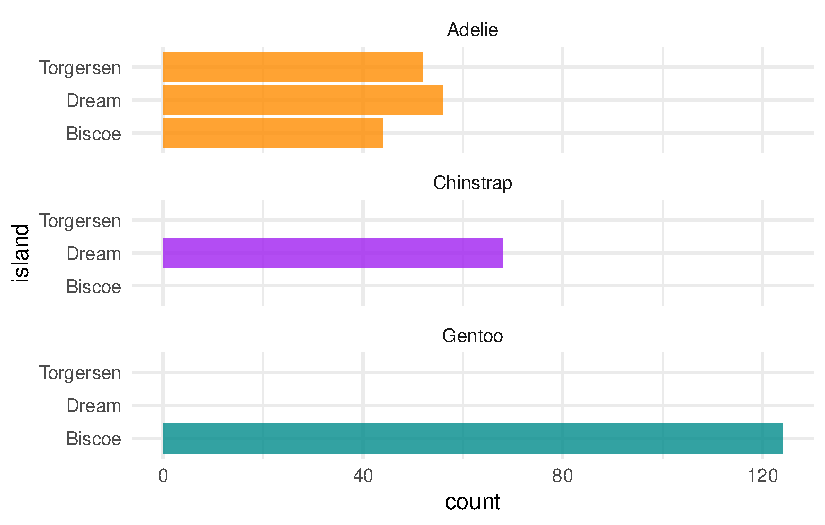
\includegraphics{paper_files/figure-pdf/fig-bills-1.pdf}

}

\caption{\label{fig-bills}Bills of penguins}

\end{figure}%

In addition to penguin data, a scatter plot below shows the relationship
between width and length of the penguins which allows us to analyze
furthermore.

\begin{figure}

\centering{

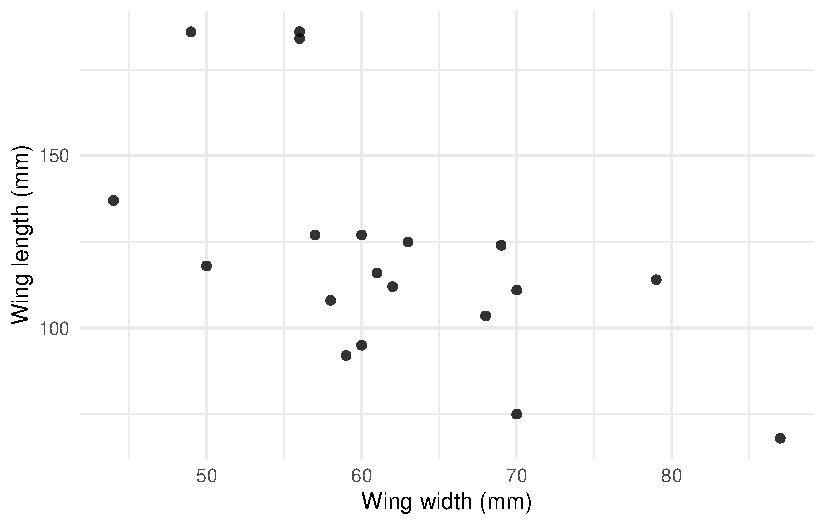
\includegraphics{paper_files/figure-pdf/fig-planes-1.pdf}

}

\caption{\label{fig-planes}Relationship between wing length and width}

\end{figure}%

This scatter plot below takes two variables which are weight and flying
time of the penguins. By observing the distribution we can notice the
relationship between weight and flying time. Therefore, observing how
likely the weight would affect the flying time.

\begin{Shaded}
\begin{Highlighting}[]
\NormalTok{simulated\_data }\OtherTok{\textless{}{-}} \FunctionTok{read\_csv}\NormalTok{(here}\SpecialCharTok{::}\FunctionTok{here}\NormalTok{(}\StringTok{"/Users/nguyenviet/Documents/STA304 {-} paper 1/data/raw\_data/simulated\_data.csv"}\NormalTok{))}
\end{Highlighting}
\end{Shaded}

\begin{verbatim}
Rows: 100 Columns: 2
-- Column specification --------------------------------------------------------
Delimiter: ","
dbl (2): flying_time, weight

i Use `spec()` to retrieve the full column specification for this data.
i Specify the column types or set `show_col_types = FALSE` to quiet this message.
\end{verbatim}

\begin{Shaded}
\begin{Highlighting}[]
\NormalTok{simulated\_data }\SpecialCharTok{|\textgreater{}}
  \FunctionTok{ggplot}\NormalTok{(}\FunctionTok{aes}\NormalTok{(}\AttributeTok{x =}\NormalTok{ weight, }\AttributeTok{y =}\NormalTok{ flying\_time)) }\SpecialCharTok{+}
  \FunctionTok{geom\_point}\NormalTok{(}\AttributeTok{alpha =} \FloatTok{0.5}\NormalTok{) }\SpecialCharTok{+}
  \FunctionTok{theme\_minimal}\NormalTok{() }\SpecialCharTok{+}
  \FunctionTok{labs}\NormalTok{(}\AttributeTok{x =} \StringTok{"weight"}\NormalTok{, }\AttributeTok{y =} \StringTok{"flying time"}\NormalTok{)}
\end{Highlighting}
\end{Shaded}

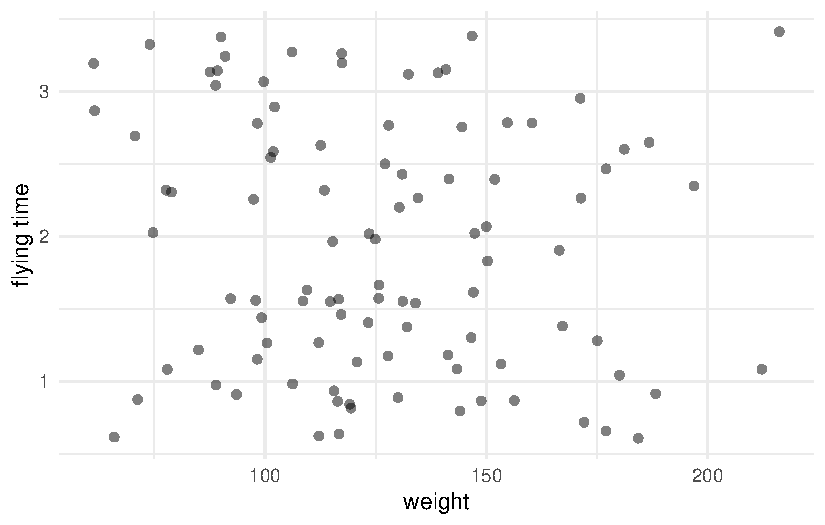
\includegraphics{paper_files/figure-pdf/unnamed-chunk-4-1.pdf}

\section{Model}\label{model}

The goal of our modelling strategy is twofold. Firstly, we aim to
investigate the relationship between weight and flying time in penguins,
contributing to a deeper understanding of how physical characteristics
impact their flight dynamics. Secondly, we have developed a simulation
model to create synthetic data that allows us to explore these
relationships under controlled conditions.

To simulate our data set, I generated 100 samples for two key variables:
flying time and weight. The flying time was derived from a uniform
distribution on the existing flying time data in our analysis data,
ensuring that the simulated values lie within the range of observed
values.

For the weight varible, I generated values from a normal distribution,
utilizing the mean and standard deviation of the length variable in the
analysis data. This decision was made based on the assumption that
weight might ahve a distribution pattern that is reflective of the
lengths of the penguins in our data set.

Here we briefly describe the Bayesian analysis model used to
investigate\ldots{} Background details and diagnostics are included in
Appendix~\ref{sec-model-details}.

\subsection{Model set-up}\label{model-set-up}

We aim to establish a statistical model that explains the variation in
flying time based on the simulated weight of penguins. The relationship
can be formally described as:
\begin{align} y_i &= \beta_0 + \beta_1 \cdot \text{weight}_i + \epsilon_i \ \epsilon_i &\sim \mbox{Normal}(0, \sigma) \end{align}

y\_i is the flying time for the ith penguin \beta\_0 is the intercept,
\beta\_1 represents the effect of weight on flying time, \epsilon\_i is
the error term, assumed to be normally distributed

Define \(y_i\) as the number of seconds that the plane remained aloft.
Then \(\beta_i\) is the wing width and \(\gamma_i\) is the wing length,
both measured in millimeters.

\begin{align} 
y_i|\mu_i, \sigma &\sim \mbox{Normal}(\mu_i, \sigma) \\
\mu_i &= \alpha + \beta_i + \gamma_i\\
\alpha &\sim \mbox{Normal}(0, 2.5) \\
\beta &\sim \mbox{Normal}(0, 2.5) \\
\gamma &\sim \mbox{Normal}(0, 2.5) \\
\sigma &\sim \mbox{Exponential}(1)
\end{align}

We run the model in R (R Core Team 2023) using the \texttt{rstanarm}
package of Goodrich et al. (2022). We use the default priors from
\texttt{rstanarm}.

\subsubsection{Model justification}\label{model-justification}

We expect a positive relationship between the size of the wings and time
spent aloft. In particular\ldots{}

We can use maths by including latex between dollar signs, for instance
\(\theta\).

\section{Results}\label{results}

Our results are summarized in Table~\ref{tbl-modelresults}.

\begin{table}

\caption{\label{tbl-modelresults}Explanatory models of flight time based
on wing width and wing length}

\centering{

\centering
\begin{tblr}[         %% tabularray outer open
]                     %% tabularray outer close
{                     %% tabularray inner open
colspec={Q[]Q[]},
column{1}={halign=l,},
column{2}={halign=c,},
hline{8}={1,2}{solid, 0.05em, black},
}                     %% tabularray inner close
\toprule
& First model \\ \midrule %% TinyTableHeader
(Intercept) & \num{1.12}    \\
& (\num{1.70})  \\
length      & \num{0.01}    \\
& (\num{0.01})  \\
width       & \num{-0.01}   \\
& (\num{0.02})  \\
Num.Obs.    & \num{19}      \\
R2          & \num{0.320}   \\
R2 Adj.     & \num{0.019}   \\
Log.Lik.    & \num{-18.128} \\
ELPD        & \num{-21.6}   \\
ELPD s.e.   & \num{2.1}     \\
LOOIC       & \num{43.2}    \\
LOOIC s.e.  & \num{4.3}     \\
WAIC        & \num{42.7}    \\
RMSE        & \num{0.60}    \\
\bottomrule
\end{tblr}

}

\end{table}%

\begin{Shaded}
\begin{Highlighting}[]
\FunctionTok{lm}\NormalTok{(flying\_time }\SpecialCharTok{\textasciitilde{}}\NormalTok{ weight, }\AttributeTok{data=}\NormalTok{simulated\_data)}
\end{Highlighting}
\end{Shaded}

\begin{verbatim}

Call:
lm(formula = flying_time ~ weight, data = simulated_data)

Coefficients:
(Intercept)       weight  
   2.276291    -0.002813  
\end{verbatim}

\section{Discussion}\label{discussion}

\subsection{First discussion point}\label{sec-first-point}

If my paper were 10 pages, then should be be at least 2.5 pages. The
discussion is a chance to show off what you know and what you learnt
from all this.

\subsection{Second discussion point}\label{second-discussion-point}

\subsection{Third discussion point}\label{third-discussion-point}

\subsection{Weaknesses and next steps}\label{weaknesses-and-next-steps}

Weaknesses and next steps should also be included.

\newpage

\appendix

\section*{Appendix}\label{appendix}
\addcontentsline{toc}{section}{Appendix}

\section{Additional data details}\label{additional-data-details}

\section{Model details}\label{sec-model-details}

\subsection{Posterior predictive
check}\label{posterior-predictive-check}

In Figure~\ref{fig-ppcheckandposteriorvsprior-1} we implement a
posterior predictive check. This shows\ldots{}

In Figure~\ref{fig-ppcheckandposteriorvsprior-2} we compare the
posterior with the prior. This shows\ldots{}

\begin{figure}

\begin{minipage}{0.50\linewidth}

\centering{

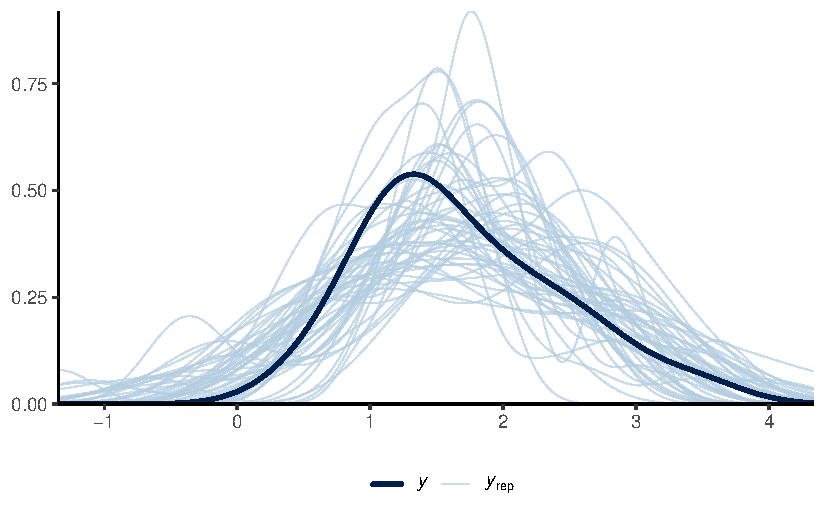
\includegraphics{paper_files/figure-pdf/fig-ppcheckandposteriorvsprior-1.pdf}

}

\subcaption{\label{fig-ppcheckandposteriorvsprior-1}Posterior prediction
check}

\end{minipage}%
%
\begin{minipage}{0.50\linewidth}

\centering{

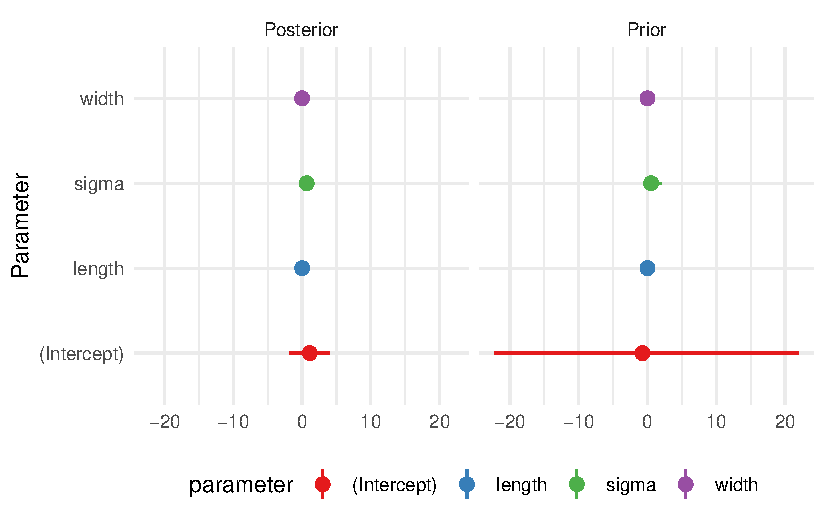
\includegraphics{paper_files/figure-pdf/fig-ppcheckandposteriorvsprior-2.pdf}

}

\subcaption{\label{fig-ppcheckandposteriorvsprior-2}Comparing the
posterior with the prior}

\end{minipage}%

\caption{\label{fig-ppcheckandposteriorvsprior}Examining how the model
fits, and is affected by, the data}

\end{figure}%

\subsection{Diagnostics}\label{diagnostics}

Figure~\ref{fig-stanareyouokay-1} is a trace plot. It shows\ldots{} This
suggests\ldots{}

Figure~\ref{fig-stanareyouokay-2} is a Rhat plot. It shows\ldots{} This
suggests\ldots{}

\begin{figure}

\begin{minipage}{0.50\linewidth}

\centering{

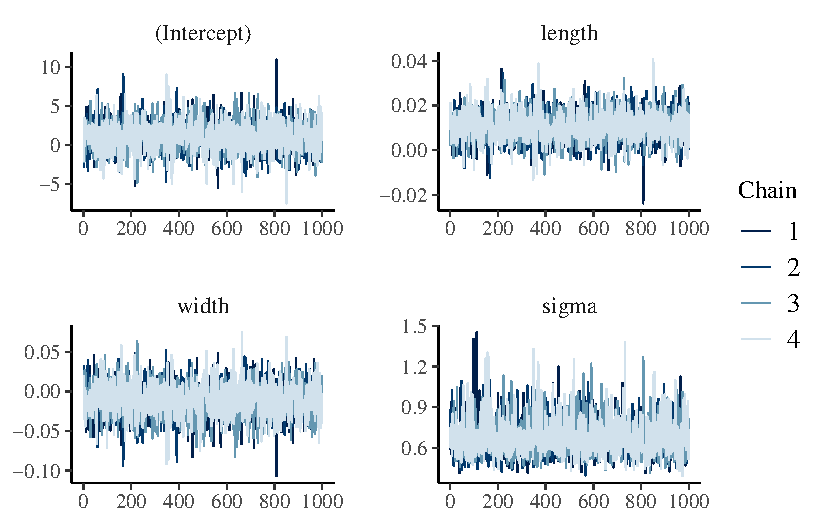
\includegraphics{paper_files/figure-pdf/fig-stanareyouokay-1.pdf}

}

\subcaption{\label{fig-stanareyouokay-1}Trace plot}

\end{minipage}%
%
\begin{minipage}{0.50\linewidth}

\centering{

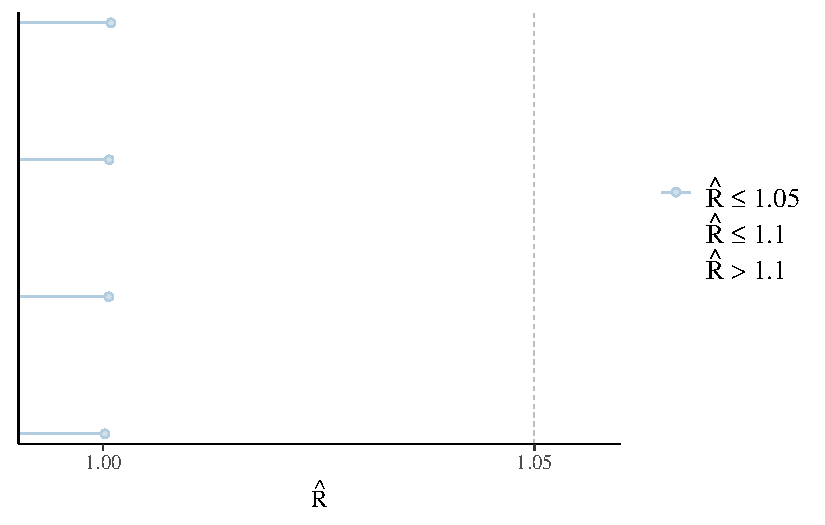
\includegraphics{paper_files/figure-pdf/fig-stanareyouokay-2.pdf}

}

\subcaption{\label{fig-stanareyouokay-2}Rhat plot}

\end{minipage}%

\caption{\label{fig-stanareyouokay}Checking the convergence of the MCMC
algorithm}

\end{figure}%

\newpage

\section*{References}\label{references}
\addcontentsline{toc}{section}{References}

\phantomsection\label{refs}
\begin{CSLReferences}{1}{0}
\bibitem[\citeproctext]{ref-rstanarm}
Goodrich, Ben, Jonah Gabry, Imad Ali, and Sam Brilleman. 2022.
{``Rstanarm: {Bayesian} Applied Regression Modeling via {Stan}.''}
\url{https://mc-stan.org/rstanarm/}.

\bibitem[\citeproctext]{ref-palmerpenguins}
Horst, Allison Marie, Alison Presmanes Hill, and Kristen B Gorman. 2020.
\emph{Palmerpenguins: Palmer Archipelago (Antarctica) Penguin Data}.
\url{https://doi.org/10.5281/zenodo.3960218}.

\bibitem[\citeproctext]{ref-citeR}
R Core Team. 2023. \emph{R: A Language and Environment for Statistical
Computing}. Vienna, Austria: R Foundation for Statistical Computing.
\url{https://www.R-project.org/}.

\end{CSLReferences}




\end{document}
